\documentclass{beamer}
\usepackage{multimedia}

\usetheme{Berlin}
\title{Pedestrain Tracking}
\author{Zhengrong Wang, Hsienyu Meng, Liuyang Zhan}
\date{\today}
\begin{document}
\begin{frame}
\titlepage
\end{frame}

\section*{Outline}
\begin{frame}
\tableofcontents
\end{frame}

\section{Introduction}

\section{Detection}
\subsection{HOG + Adaboost}
\begin{frame}
\frametitle{HOG + Adaboost}
\begin{itemize}
\item Offline trained Adaboost classifier with 20 layers.
\item Each layer contains variable number of weak classifiers.
\item Each weak classifier calculates the HOG feature of a small patch in the ROI.
\item ($2\times2$ subregions) $\times$ (9 bins for HOG) = feature vector of 36 dimension.
\item Sliding windows and non-maximum suppression to detect pedestrain.
\end{itemize}
\end{frame}

\subsection{Background Subtraction}
\begin{frame}
\frametitle{Background Subtraction}
\begin{itemize}
\item Mean-shift to construct background model.
\item Subtracting background from the current model.
\item Find the connected components.
\begin{itemize}
	\item Label as pedestrain if it satisfys some criterions.
	\item Use Adaboost classifier for further detection.

\end{itemize}
\end{itemize}
\end{frame}

\subsection{Results}
\begin{frame}
	\frametitle{Results}
	\begin{columns}[T]
		\begin{column}{.5\textwidth}
		\begin{figure}
		\begin{center}
			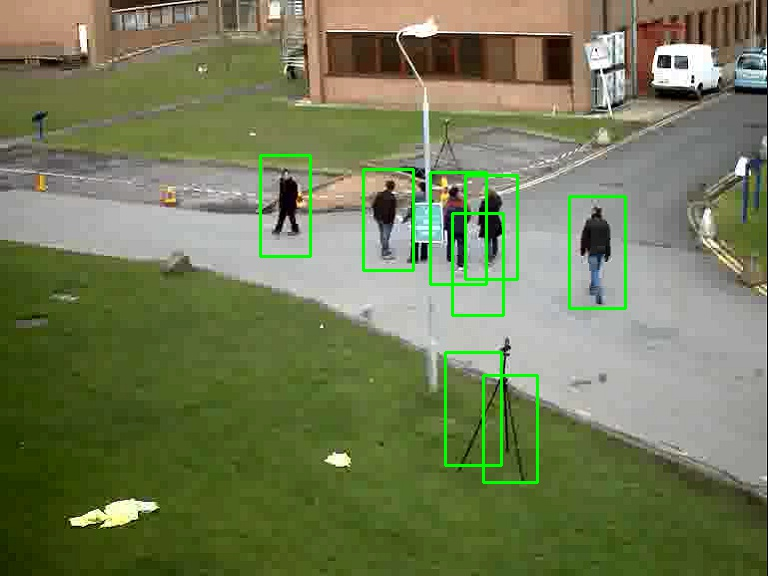
\includegraphics[width=\textwidth]{images/ImageDetector.jpg}
			\caption{HOG Detection Results}
			\label{fig:sub:ImageDetector}
		\end{center}
		\end{figure}
		\end{column}
		\begin{column}{.5\textwidth}
		\begin{figure}
		\begin{center}
			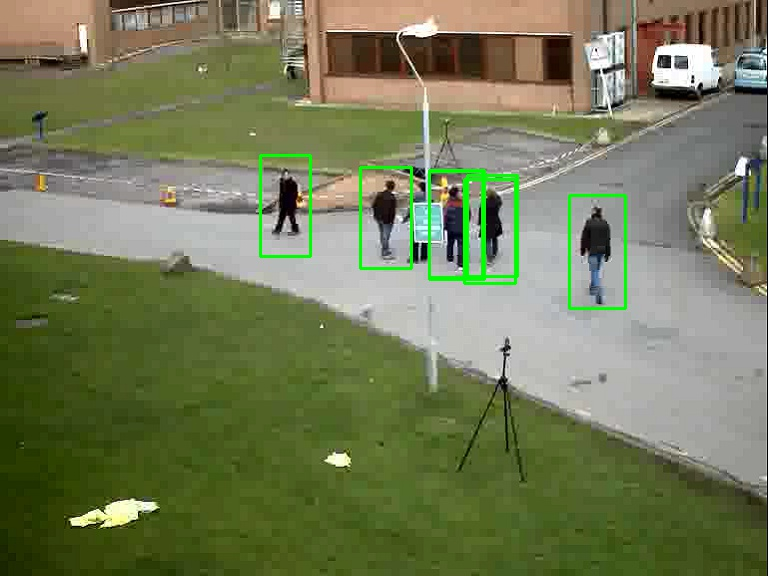
\includegraphics[width=\textwidth]{images/BKGCutDetector.jpg}
			\caption{BKG Subtraction Results}
			\label{fig:sub:BKGCutDetector}
		\end{center}
		\end{figure}
		\end{column}
	\end{columns}
\end{frame}

\section{Tracking}
\subsection{Particle Filter}
\begin{frame}
	\frametitle{Particle Fitler}
	\begin{columns}[T]
		\begin{column}{0.7\textwidth}
		\begin{figure}
		\begin{center}
			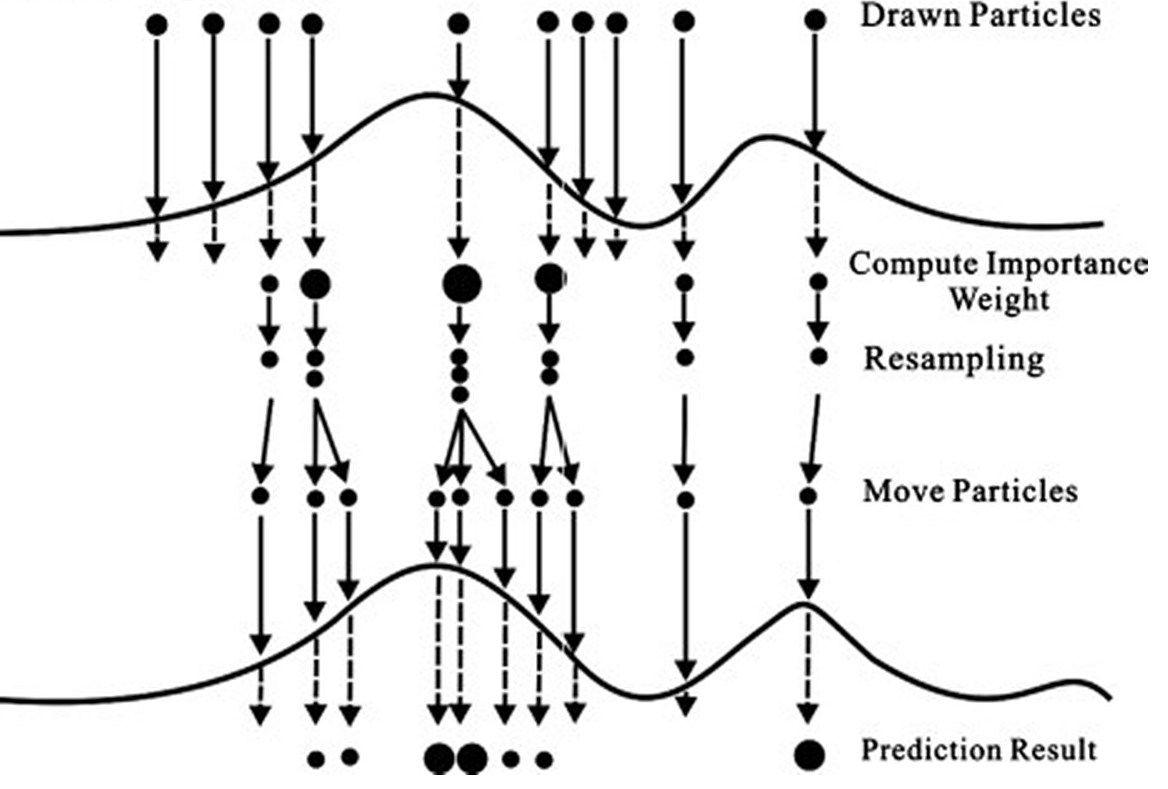
\includegraphics[width=0.8\textwidth]{images/particlefilter.png}
			\caption{Particle Filters}
		\end{center}
		\end{figure}
		\end{column}
		\begin{column}{0.3\textwidth}
			\begin{itemize}
				\item Propagate.
				\item Observe.
				\item Resample.
			\end{itemize}
		\end{column}
	\end{columns}
\end{frame}

\begin{frame}
	\frametitle{Particle Filter with Constant Velocity}
	\begin{itemize}
		\item Propagate.
		\begin{align}
		x_{t}&=x_{t-1}+v_{t-1}+N(0, \sigma_x)\\
		v_{t}&=v_{t-1}+N(0, \sigma_v)
		\end{align}

		\item Observe.
		\begin{itemize}
		\item Online boosting classifier.
		\item Matched detection.
		\end{itemize}
		\item Resample.\\
		Resample with the weights calculated in previous stage.
	\end{itemize}
\end{frame}

\subsection{Online Boosting Classifier}
\begin{frame}
	\frametitle{Online Boosting Classifier}
	\begin{columns}[T]
		\begin{column}{0.6\textwidth}
		\begin{figure}
		\begin{center}
			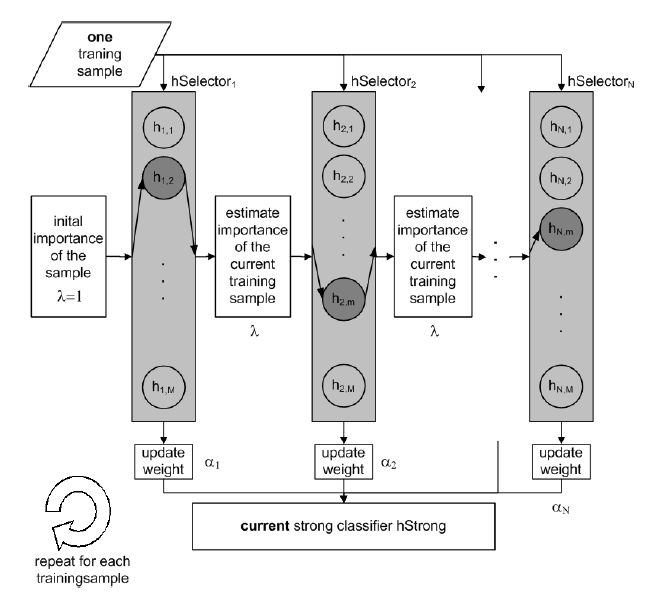
\includegraphics[width=0.7\textwidth]{images/OnlineBoosting.png}
			\caption{Online Boosting}
		\end{center}
		\end{figure}
		\end{column}
		\begin{column}{0.4\textwidth}
			\begin{itemize}
				\item Weak classifier pool.
				\item Selectors.
				\item Strong classifier.
			\end{itemize}
		\end{column}
	\end{columns}
\end{frame}

\begin{frame}
	\frametitle{Weak Classifier}
	\begin{itemize}
		\item Each weak classifier evaluates a feature.
		\item Uses Kalman filter to estimate the Gaussian distribution of positive and negative features.
		\begin{align}
			K_{t}&=\frac{P_{t-1}}{P_{t-1}+R}\\
			\mathbf{\mu}_{t}&=K_{t}f(\mathbf{x})+(1-K_{t})\mathbf{\mu}_{t-1}\\
			\mathbf{\sigma}_{t}^{2}&=K_{t}(f(\mathbf{x})-\mathbf{\mu}_{t})^{2}+(1-K_{t})\mathbf{\sigma}_{t-1}^{2}\\
			P_{t}&=(1-K_{t})P_{t-1}
		\end{align}
		\item A simple Eculidean distance threshold is enough to generate the hyposis.
		\begin{equation}
			h(\mathbf{x})=\min_{+, -}(D(f(\mathbf{x}), \mu_{+}), D(f(\mathbf{x}), \mu_{-}))
		\end{equation}
	\end{itemize}
\end{frame}

\begin{frame}
	\frametitle{Selector}
	\begin{itemize}
		\item Evaluates the error rate of a weak classifier by:
		\begin{equation}
			err\approx\frac{\lambda_{wrong}}{\lambda_{wrong}+\lambda_{correct}}
		\end{equation}
		\item For each training, selects the best weak classifier, and replaces the worst classifier with a newly initialized one.
		\item A cycle queue for backup of weak classifiers.
		\begin{figure}
			\begin{center}
			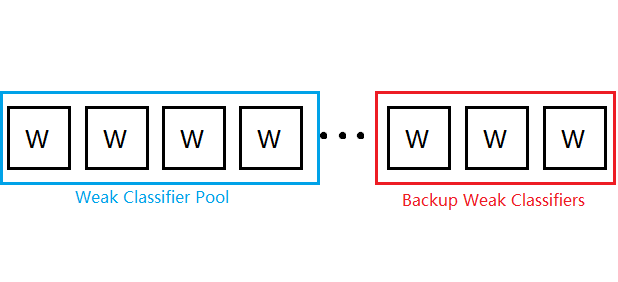
\includegraphics[width=0.8\textwidth]{images/WeakClassifierPool.png}
			\caption{Weak Classifier Pool}
			\end{center}
		\end{figure}
	\end{itemize}
\end{frame}

\begin{frame}
	\frametitle{Strong Classifier}
	\begin{itemize}
		\item Cascade of selectors is a strong classifier.
		\item The final output is given by:
		\begin{equation}
			h^{strong}(\mathbf{x})=\mathrm{sign}(\sum_{i=1}^{N}\alpha_{i}\cdot h^{selector}_{i}(\mathbf{x}))
		\end{equation}
		\item $\alpha$ is the weight of each selector given by:
		\begin{equation}
			\alpha_i=\ln(\frac{1-err_i}{err_i})
		\end{equation}
	\end{itemize}
\end{frame}

\subsection{Single Target Tracking}
\begin{frame}
	\frametitle{Single Target Tracking}
	\begin{enumerate}
		\item Initialize the target.
		\item Propagate the particles.
		\item Make observation.
		\item Resample the particles, and find the target.
		\item Sample around the new position and train the online boosting classifier. Go back to Step~2.
	\end{enumerate}
\end{frame}

\begin{frame}
	\frametitle{Results}
	\begin{columns}[T]
		\begin{column}{0.5\textwidth}
		Grayscale Haar-like feature.
		\begin{center}
			\movie[once, poster,externalviewer]{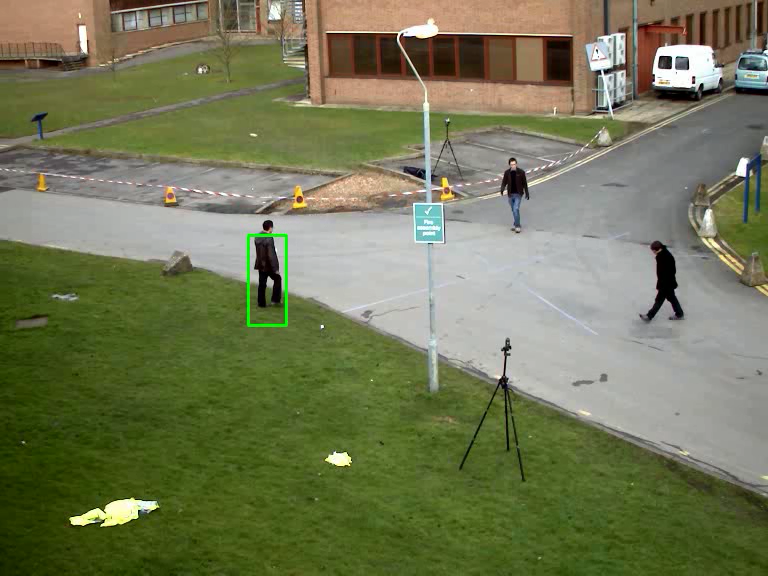
\includegraphics[width=\textwidth]{video/singlePoster.png}}{video/singleTrackerTestGray01.avi}
		\end{center}
		\end{column}
		\begin{column}{0.5\textwidth}
		RedGreenIntensity feature.
		\begin{center}
			\movie[once, poster,externalviewer]{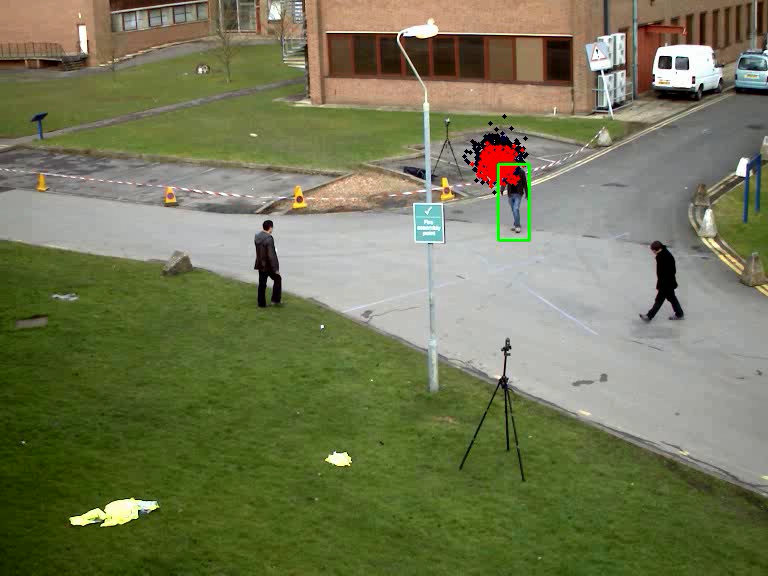
\includegraphics[width=\textwidth]{video/rgiPoster.png}}{video/singleTrackerTestRGI01.avi}
		\end{center}
		\end{column}
	\end{columns}
\end{frame}

\subsection{Multiple Targets Tracking}
\begin{frame}
	\frametitle{Multiple Targets Tracking}
	\begin{itemize}
		\item Data Association Problem
		\begin{itemize}
			\item Match matrix with score:

			\item Greedy algorithm to find the match.
		\end{itemize}
		\item Occlusion
		\begin{itemize}
			\item Depth field.
			\item Occlusion reasoning.		
		\end{itemize}
	\end{itemize}
\end{frame}

\begin{frame}
	\frametitle{Results}
	\begin{columns}[T]
		\begin{column}{0.5\textwidth}
			\begin{figure}
				\begin{center}
					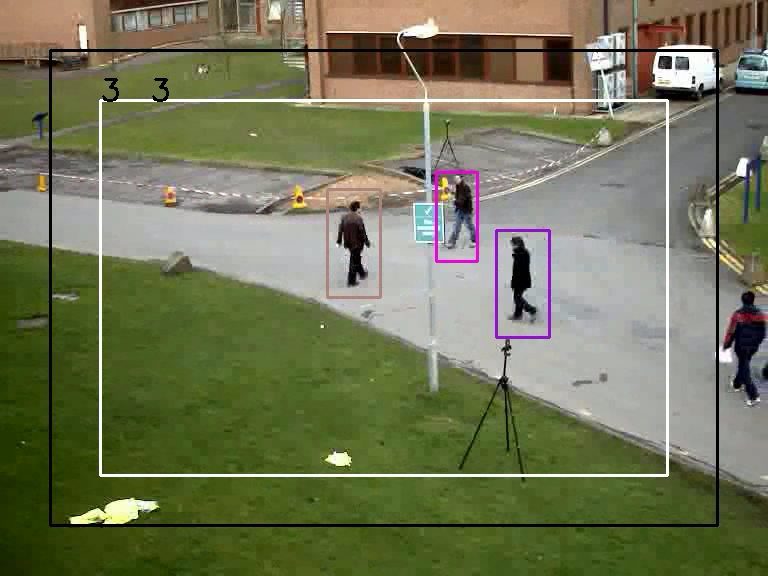
\includegraphics[width=\textwidth]{images/MultiTrackerInit01.png}
					\caption{Multiple Tracker Initialized}
				\end{center}
			\end{figure}
		\end{column}
		\begin{column}{0.5\textwidth}
			\begin{figure}
				\begin{center}
					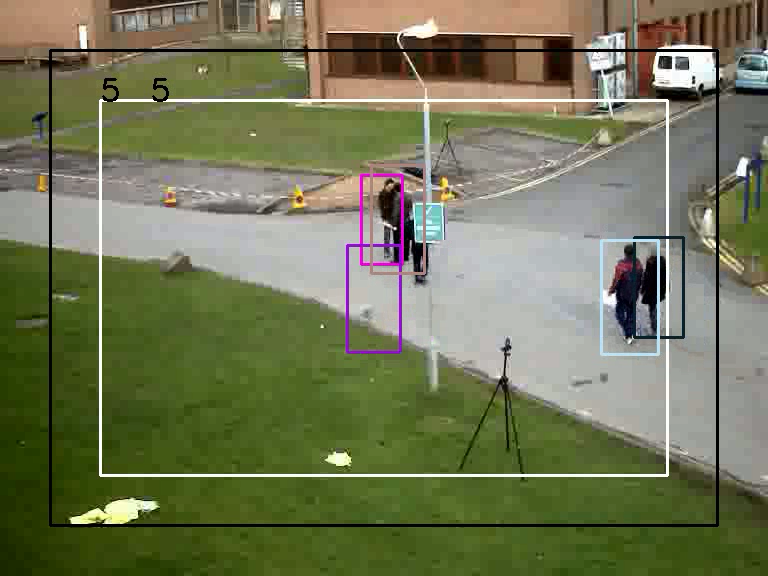
\includegraphics[width=\textwidth]{images/MultiTrackerLost01.png}
					\caption{Multiple Tracker Lost}
				\end{center}
			\end{figure}
		\end{column}
	\end{columns}
\end{frame}

\begin{frame}
	\frametitle{Problems and Solutions}
	\begin{itemize}
		\item Match score should be more robustic and less dependent on the distance term.
		\item If there is occlusion, the detector may fail for many frames, The particle filter will almost certainly lose its target.
		\item With depth field this may be solved.
	\end{itemize}
\end{frame}

\subsection{Energy Minimization}
\begin{frame}
	\frametitle{Energy Minimization}
	\begin{itemize}
		\item Use Kalman filter or extended Kalman filter to get a initial solution.
		\item Optimized on a energy function within a temporal window.
		\item The result is quite good, however this method is not causal. It needs information in the future.
	\end{itemize}
	\begin{figure}
		\begin{center}
			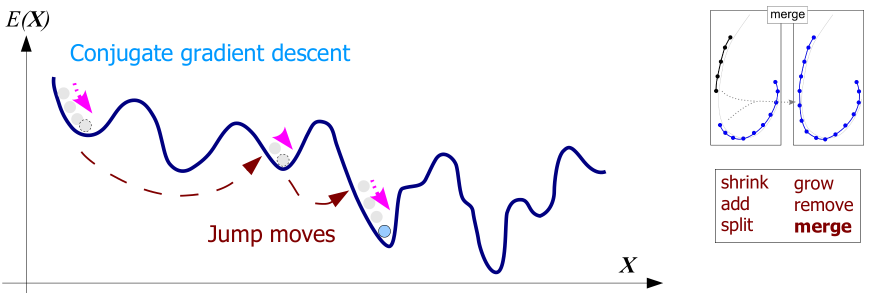
\includegraphics[width=0.7\textwidth]{images/energy.png}
			\caption{Energy Minimization}
		\end{center}
	\end{figure}
\end{frame}

\begin{frame}
	\frametitle{Results}
	\begin{center}
		\movie[once,poster,externalviewer]{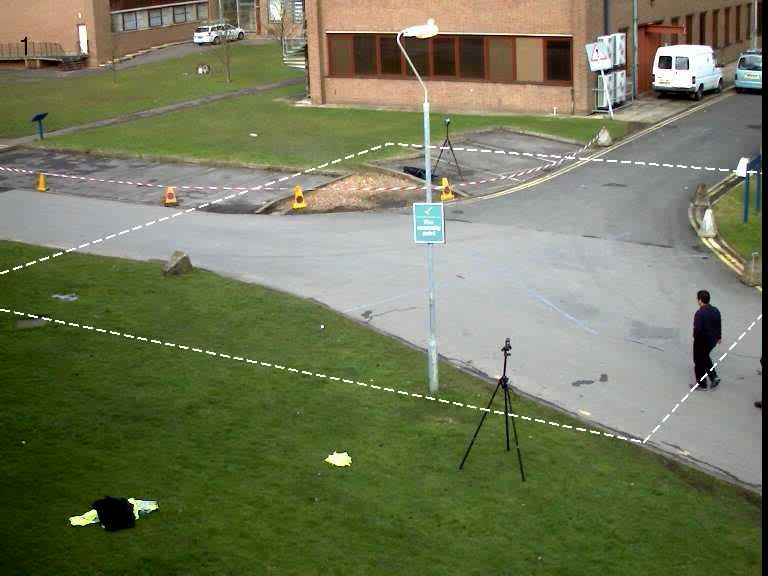
\includegraphics[width=0.7\textwidth]{video/energy.png}}{video/energy.avi}
	\end{center}
\end{frame}

\section{Summary}
\begin{frame}
	\frametitle{Summary}
	\begin{itemize}
		\item Multiple targets tracking is still a very challenging problem in computer vision.
		\item Real time? With GPU and multiple threads, this is possible.
	\end{itemize}
\end{frame}

% \begin{frame}{Bibliography}
% \bibliographystyle{plainnat}
% \bibliography{Ref}
% \end{frame}

\begin{frame}
	\frametitle{Thank you!}
	\begin{itemize}
		\item Project Website:\\
		\href{https://zerowong.github.io/PedestrainCounting/}{https://zerowong.github.io/PedestrainCounting/}
		\item GitHub Repo:\\
		\href{https://github.com/zerowong/PedestrainCounting}{https://github.com/zerowong/PedestrainCounting/}
	\end{itemize}
	\begin{figure}
		\begin{center}
			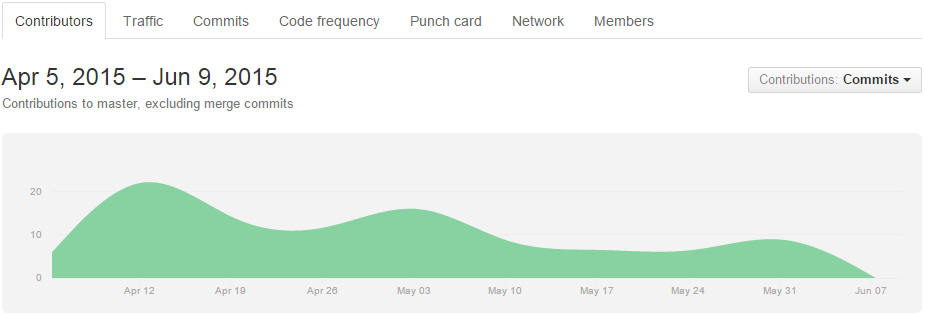
\includegraphics[width=0.9\textwidth]{images/git.png}
		\end{center}
	\end{figure}
\end{frame}

\end{document}
